\documentclass[a4paper,12pt]{article}

\usepackage[utf8x]{inputenc}
\usepackage[T2A]{fontenc}
\usepackage[english, russian]{babel}

% Опционно, требует  apt-get install scalable-cyrfonts.*
% и удаления одной строчки в cyrtimes.sty
% Сточку не удалять!
% \usepackage{cyrtimes}

% Картнки и tikz
\usepackage{graphicx}
\usepackage{tikz}
\usetikzlibrary{snakes,arrows,shapes}


% Некоторая русификация.
\usepackage{misccorr}
\usepackage{indentfirst}
\renewcommand{\labelitemi}{\normalfont\bfseries{--}}

% Увы, поля придётся уменьшить из-за листингов.
\topmargin -1cm
\oddsidemargin -0.5cm
\evensidemargin -0.5cm
\textwidth 17cm
\textheight 24cm

\sloppy

% Оглавление в PDF
\usepackage[
bookmarks=true,
colorlinks=true, linkcolor=black, anchorcolor=black, citecolor=black, menucolor=black,filecolor=black, urlcolor=black,
unicode=true
]{hyperref}

% Для исходного кода в тексте
\newcommand{\Code}[1]{\texttt{#1}}

\usepackage{verbatim}
\usepackage{fancyvrb}
\fvset{frame=leftline, fontsize=\small, framerule=0.4mm, rulecolor=\color{darkgray}, commandchars=\\\{\}}
\renewcommand{\theFancyVerbLine}{\small\arabic{FancyVerbLine}}


\title{Отчёт по лабораторной работе \\ <<IP-маршрутизация>>}
\author{Зиновьев Д.В.}

\begin{document}

\maketitle

\tableofcontents

\section{Топология сети}

Топология сети и использыемые IP-адреса показаны на рис.~\ref{fig:network}.

\begin{figure}
\centering
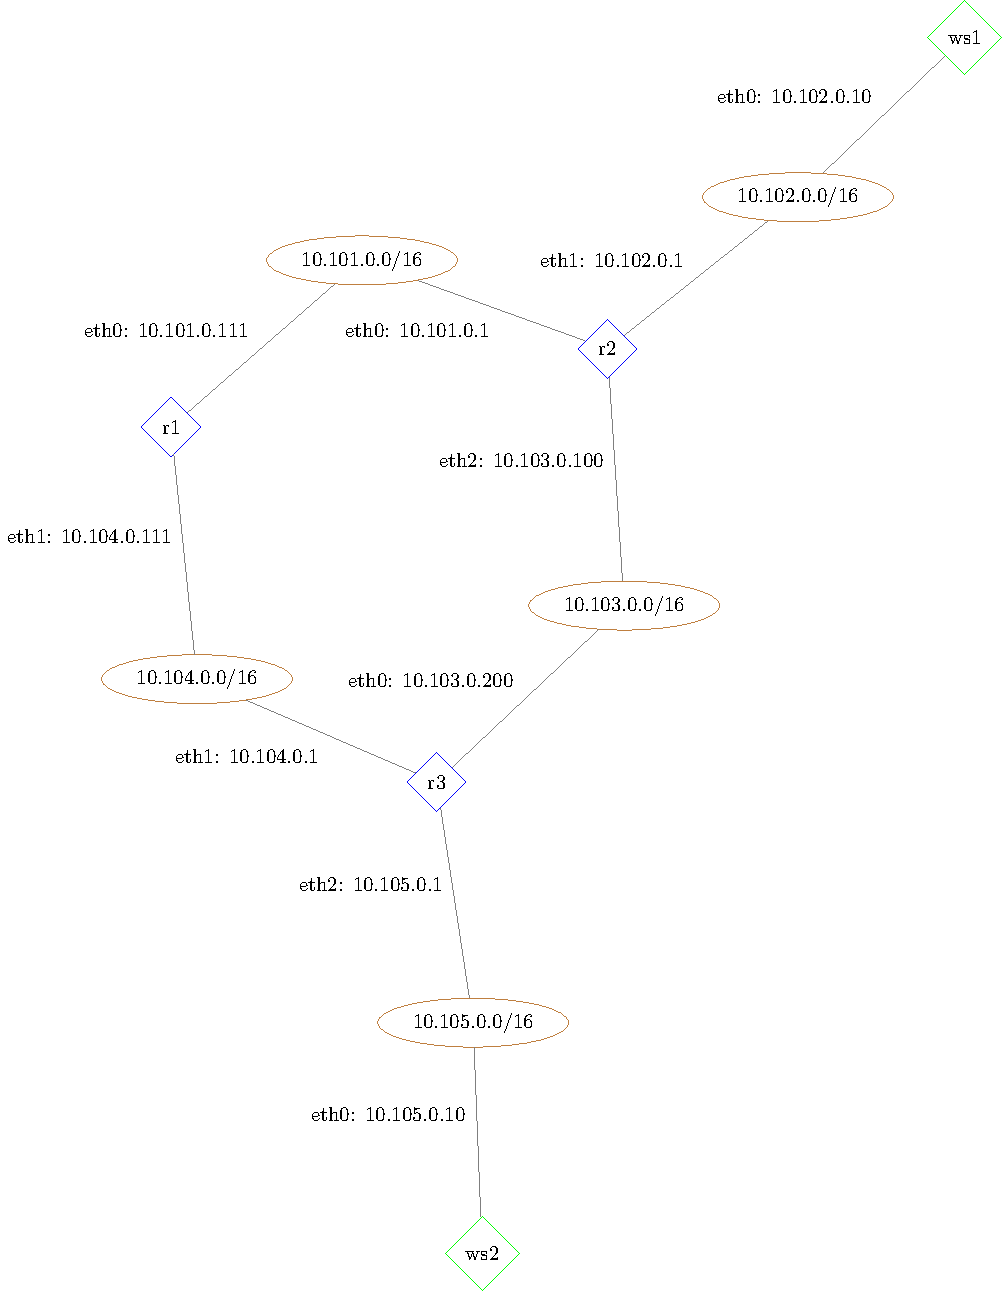
\includegraphics[width=\textwidth]{includes/network_gv.pdf}
\caption{Топология сети}
\label{fig:network}
\end{figure}


\section{Назначение IP-адресов}

Ниже приведён файл настройки протокола IP маршрутизатора \textbf{r2}.

\begin{Verbatim}
r2:~# cat /etc/network/interfaces 
auto lo
iface lo inet loopback

auto eth0
iface eth0 inet static
address 10.101.0.1
netmask 255.255.0.0

up ip r add 10.104.0.0/16 via 10.101.0.111 dev eth0
down ip r del 10.104.0.0/16

auto eth1
iface eth1 inet static
address 10.102.0.1
netmask 255.255.0.0

auto eth2
iface eth2 inet static
address 10.103.0.100
netmask 255.255.0.0

up ip r add 10.105.0.0/16 via 10.103.0.200 dev eth2
down ip r del 10.105.0.0/16
\end{Verbatim}

Ниже приведён файл настройки протокола IP рабочей станции \textbf{ws1}.

\begin{Verbatim}
ws1:~# cat /etc/network/interfaces 
auto lo
iface lo inet loopback

auto eth0
iface eth0 inet static
address 10.102.0.10
netmask 255.255.0.0
gateway 10.102.0.1
\end{Verbatim}


\section{Таблица маршрутизации}

Таблица маршрутизации для \textbf{r1}.

\begin{Verbatim}
r1:~# ip r
10.101.0.0/16 dev eth0  proto kernel  scope link  src 10.101.0.111 
10.103.0.0/16 via 10.101.0.1 dev eth0 
10.102.0.0/16 via 10.101.0.1 dev eth0 
10.105.0.0/16 via 10.104.0.1 dev eth1 
10.104.0.0/16 dev eth1  proto kernel  scope link  src 10.104.0.111
\end{Verbatim}

Таблица маршрутизации для \textbf{r2}.

\begin{Verbatim}
r2:~# ip r
10.101.0.0/16 dev eth0  proto kernel  scope link  src 10.101.0.1 
10.103.0.0/16 dev eth2  proto kernel  scope link  src 10.103.0.100 
10.102.0.0/16 dev eth1  proto kernel  scope link  src 10.102.0.1 
10.105.0.0/16 via 10.103.0.200 dev eth2 
10.104.0.0/16 via 10.101.0.111 dev eth0
\end{Verbatim}

Таблица маршрутизации для \textbf{r3}.

\begin{Verbatim}
r3:~# ip r
10.101.0.0/16 via 10.103.0.100 dev eth0 
10.103.0.0/16 dev eth0  proto kernel  scope link  src 10.103.0.200 
10.102.0.0/16 via 10.103.0.100 dev eth0 
10.105.0.0/16 dev eth2  proto kernel  scope link  src 10.105.0.1 
10.104.0.0/16 dev eth1  proto kernel  scope link  src 10.104.0.1
\end{Verbatim}


\section{Проверка настройки сети}

Вывод \textbf{traceroute} от узла \textbf{ws1} до \textbf{r1} при нормальной работе сети.

\begin{Verbatim}
ws1:~# traceroute 10.101.0.111
traceroute to 10.101.0.111 (10.101.0.111), 64 hops max, 40 byte packets
 1  10.102.0.1 (10.102.0.1)  0 ms  0 ms  0 ms
 2  10.101.0.111 (10.101.0.111)  0 ms  0 ms  0 ms
ws1:~# traceroute 10.104.0.111
traceroute to 10.104.0.111 (10.104.0.111), 64 hops max, 40 byte packets
 1  10.102.0.1 (10.102.0.1)  1 ms  1 ms  0 ms
 2  10.104.0.111 (10.104.0.111)  1 ms  1 ms  1 ms
\end{Verbatim}

Вывод \textbf{traceroute} от узла \textbf{ws1} до \textbf{r2} при нормальной работе сети.

\begin{Verbatim}
ws1:~# traceroute 10.101.0.1
traceroute to 10.101.0.1 (10.101.0.1), 64 hops max, 40 byte packets
 1  10.101.0.1 (10.101.0.1)  11 ms  1 ms  0 ms
ws1:~# traceroute 10.102.0.1
traceroute to 10.102.0.1 (10.102.0.1), 64 hops max, 40 byte packets
 1  10.102.0.1 (10.102.0.1)  1 ms  1 ms  0 ms
ws1:~# traceroute 10.103.0.100
traceroute to 10.103.0.100 (10.103.0.100), 64 hops max, 40 byte packets
 1  10.103.0.100 (10.103.0.100)  0 ms  0 ms  0 ms
\end{Verbatim}

Вывод \textbf{traceroute} от узла \textbf{ws1} до \textbf{r3} при нормальной работе сети.

\begin{Verbatim}
ws1:~# traceroute 10.103.0.200
traceroute to 10.103.0.200 (10.103.0.200), 64 hops max, 40 byte packets
 1  10.102.0.1 (10.102.0.1)  0 ms  0 ms  0 ms
 2  10.103.0.200 (10.103.0.200)  11 ms  0 ms  0 ms
ws1:~# traceroute 10.104.0.1
traceroute to 10.104.0.1 (10.104.0.1), 64 hops max, 40 byte packets
 1  10.102.0.1 (10.102.0.1)  0 ms  0 ms  0 ms
 2  10.101.0.111 (10.101.0.111)  0 ms  0 ms  0 ms
 3  10.104.0.1 (10.104.0.1)  11 ms  1 ms  1 ms
ws1:~# traceroute 10.105.0.1
traceroute to 10.105.0.1 (10.105.0.1), 64 hops max, 40 byte packets
 1  10.102.0.1 (10.102.0.1)  0 ms  0 ms  0 ms
 2  10.105.0.1 (10.105.0.1)  0 ms  0 ms  0 ms
\end{Verbatim}

Вывод \textbf{traceroute} от узла \textbf{ws1} до \textbf{ws2} при нормальной работе сети.

\begin{Verbatim}
ws1:~# traceroute 10.105.0.10
traceroute to 10.105.0.10 (10.105.0.10), 64 hops max, 40 byte packets
 1  10.102.0.1 (10.102.0.1)  0 ms  0 ms  0 ms
 2  10.103.0.200 (10.103.0.200)  0 ms  0 ms  0 ms
 3  10.105.0.10 (10.105.0.10)  0 ms  0 ms  0 ms
\end{Verbatim}

Вывод \textbf{traceroute} от узла \textbf{ws2} до \textbf{r1} при нормальной работе сети.

\begin{Verbatim}
ws2:~# traceroute 10.101.0.111
traceroute to 10.101.0.111 (10.101.0.111), 64 hops max, 40 byte packets
 1  10.105.0.1 (10.105.0.1)  1 ms  0 ms  0 ms
 2  10.103.0.100 (10.103.0.100)  0 ms  0 ms  1 ms
 3  10.101.0.111 (10.101.0.111)  1 ms  1 ms  1 ms
ws2:~# traceroute 10.104.0.111
traceroute to 10.104.0.111 (10.104.0.111), 64 hops max, 40 byte packets
 1  10.105.0.1 (10.105.0.1)  0 ms  0 ms  0 ms
 2  10.104.0.111 (10.104.0.111)  0 ms  0 ms  0 ms
\end{Verbatim}

Вывод \textbf{traceroute} от узла \textbf{ws2} до \textbf{r2} при нормальной работе сети.

\begin{Verbatim}
ws2:~# traceroute 10.101.0.1
traceroute to 10.101.0.1 (10.101.0.1), 64 hops max, 40 byte packets
 1  10.105.0.1 (10.105.0.1)  0 ms  0 ms  0 ms
 2  10.101.0.1 (10.101.0.1)  0 ms  0 ms  0 ms
ws2:~# traceroute 10.102.0.1
traceroute to 10.102.0.1 (10.102.0.1), 64 hops max, 40 byte packets
 1  10.105.0.1 (10.105.0.1)  0 ms  0 ms  0 ms
 2  10.102.0.1 (10.102.0.1)  0 ms  0 ms  0 ms
ws2:~# traceroute 10.103.0.100
traceroute to 10.103.0.100 (10.103.0.100), 64 hops max, 40 byte packets
 1  10.105.0.1 (10.105.0.1)  0 ms  0 ms  0 ms
 2  10.103.0.100 (10.103.0.100)  0 ms  0 ms  0 ms
\end{Verbatim}

Вывод \textbf{traceroute} от узла \textbf{ws2} до \textbf{r3} при нормальной работе сети.

\begin{Verbatim}
ws2:~# traceroute 10.103.0.200
traceroute to 10.103.0.200 (10.103.0.200), 64 hops max, 40 byte packets
 1  10.103.0.200 (10.103.0.200)  0 ms  0 ms  0 ms
ws2:~# traceroute 10.104.0.1
traceroute to 10.104.0.1 (10.104.0.1), 64 hops max, 40 byte packets
 1  10.104.0.1 (10.104.0.1)  0 ms  0 ms  0 ms
ws2:~# traceroute 10.105.0.1
traceroute to 10.105.0.1 (10.105.0.1), 64 hops max, 40 byte packets
 1  10.105.0.1 (10.105.0.1)  1 ms  1 ms  0 ms
\end{Verbatim}

Вывод \textbf{traceroute} от узла \textbf{ws2} до \textbf{ws1} при нормальной работе сети.

\begin{Verbatim}
ws2:~# traceroute 10.102.0.10
traceroute to 10.102.0.10 (10.102.0.10), 64 hops max, 40 byte packets
 1  10.105.0.1 (10.105.0.1)  0 ms  0 ms  0 ms
 2  10.103.0.100 (10.103.0.100)  0 ms  0 ms  0 ms
 3  10.102.0.10 (10.102.0.10)  0 ms  0 ms  0 ms
\end{Verbatim}


\section{Маршрутизация}

MAC-адреса интерфейсов для \textbf{ws1}.

\begin{Verbatim}
ws1:~# ifconfig -a | grep 'eth.*' | awk {'printf("%s %s", $1, $5)'}
eth0 a6:f9:52:b6:1e:69
\end{Verbatim}

MAC-адреса интерфейсов для \textbf{ws2}.

\begin{Verbatim}
ws2:~# ifconfig -a | grep 'eth.*' | awk {'printf("%s %s", $1, $5)'}
eth0 da:53:12:09:ea:4e
\end{Verbatim}

MAC-адреса интерфейсов для \textbf{r1}.

\begin{Verbatim}
r1:~# ifconfig -a | grep 'eth.*' | awk {'printf("%s %s", $1, $5)'}
eth0 0e:ab:f8:0c:10:4b
eth1 fa:de:dc:30:96:57
\end{Verbatim}

MAC-адреса интерфейсов для \textbf{r2}.

\begin{Verbatim}
r2:~# ifconfig -a | grep 'eth.*' | awk {'printf("%s %s", $1, $5)'}
eth0 3a:40:ee:31:9e:cd
eth1 12:3e:e2:7d:e3:87
eth2 4a:6c:31:ed:d1:db
\end{Verbatim}

MAC-адреса интерфейсов для \textbf{r3}.

\begin{Verbatim}
r3:~# ifconfig -a | grep 'eth.*' | awk {'printf("%s %s", $1, $5)'}
eth0 ee:97:f2:ab:47:0c
eth1 d2:90:43:d2:95:19
eth2 c2:57:e2:f3:3f:00
\end{Verbatim}

Для каждого узла сети выполнена команда для очистки кеша протокола ARP.

\begin{Verbatim}
# ip n flush all
\end{Verbatim}

Отправка пакета от \textbf{ws1} к \textbf{ws2} для случая, когда ARP кеш очищен.

\begin{Verbatim}
ws1:~# ping -c 1 10.105.0.10
PING 10.105.0.10 (10.105.0.10) 56(84) bytes of data.
64 bytes from 10.105.0.10: icmp_seq=1 ttl=62 time=40.7 ms

--- 10.105.0.10 ping statistics ---
1 packets transmitted, 1 received, 0% packet loss, time 0ms
rtt min/avg/max/mdev = 40.768/40.768/40.768/0.000 ms

ws1:~# tcpdump -ntve
a6:f9:52:b6:1e:69 > ff:ff:ff:ff:ff:ff, ethertype ARP (0x0806), length 42:
    arp who-has 10.102.0.1 tell 10.102.0.10
12:3e:e2:7d:e3:87 > a6:f9:52:b6:1e:69, ethertype ARP (0x0806), length 42:
    arp reply 10.102.0.1 is-at 12:3e:e2:7d:e3:87
a6:f9:52:b6:1e:69 > 12:3e:e2:7d:e3:87, ethertype IPv4 (0x0800), length 98:
    (tos 0x0, ttl 64, id 0, offset 0, flags [DF], proto ICMP (1), length 84)
    10.102.0.10 > 10.105.0.10: ICMP echo request, id 24322, seq 1, length 64
12:3e:e2:7d:e3:87 > a6:f9:52:b6:1e:69, ethertype IPv4 (0x0800), length 98:
    (tos 0x0, ttl 62, id 34455, offset 0, flags [none], proto ICMP (1), length 84)
    10.105.0.10 > 10.102.0.10: ICMP echo reply, id 24322, seq 1, length 64

r2:~# tcpdump -ntve -i any
  B a6:f9:52:b6:1e:69 ethertype ARP (0x0806), length 44:
    arp who-has 10.102.0.1 tell 10.102.0.10
Out 12:3e:e2:7d:e3:87 ethertype ARP (0x0806), length 44:
    arp reply 10.102.0.1 is-at 12:3e:e2:7d:e3:87
 In a6:f9:52:b6:1e:69 ethertype IPv4 (0x0800), length 100:
    (tos 0x0, ttl 64, id 0, offset 0, flags [DF], proto ICMP (1), length 84)
    10.102.0.10 > 10.105.0.10: ICMP echo request, id 24322, seq 1, length 64
Out 4a:6c:31:ed:d1:db ethertype ARP (0x0806), length 44:
    arp who-has 10.103.0.200 tell 10.103.0.100
 In ee:97:f2:ab:47:0c ethertype ARP (0x0806), length 44:
    arp reply 10.103.0.200 is-at ee:97:f2:ab:47:0c
Out 4a:6c:31:ed:d1:db ethertype IPv4 (0x0800), length 100:
    (tos 0x0, ttl 63, id 0, offset 0, flags [DF], proto ICMP (1), length 84)
    10.102.0.10 > 10.105.0.10: ICMP echo request, id 24322, seq 1, length 64
 In ee:97:f2:ab:47:0c ethertype IPv4 (0x0800), length 100:
    (tos 0x0, ttl 63, id 34455, offset 0, flags [none], proto ICMP (1), length 84)
    10.105.0.10 > 10.102.0.10: ICMP echo reply, id 24322, seq 1, length 64
Out 12:3e:e2:7d:e3:87 ethertype IPv4 (0x0800), length 100:
    (tos 0x0, ttl 62, id 34455, offset 0, flags [none], proto ICMP (1), length 84)
    10.105.0.10 > 10.102.0.10: ICMP echo reply, id 24322, seq 1, length 64
Out 12:3e:e2:7d:e3:87 ethertype ARP (0x0806), length 44:
    arp who-has 10.102.0.10 tell 10.102.0.1
 In a6:f9:52:b6:1e:69 ethertype ARP (0x0806), length 44:
    arp reply 10.102.0.10 is-at a6:f9:52:b6:1e:69
 In ee:97:f2:ab:47:0c ethertype ARP (0x0806), length 44:
    arp who-has 10.103.0.100 tell 10.103.0.200
Out 4a:6c:31:ed:d1:db ethertype ARP (0x0806), length 44:
    arp reply 10.103.0.100 is-at 4a:6c:31:ed:d1:db

r3:~# tcpdump -ntve -i any
  B 4a:6c:31:ed:d1:db ethertype ARP (0x0806), length 44:
    arp who-has 10.103.0.200 tell 10.103.0.100
Out ee:97:f2:ab:47:0c ethertype ARP (0x0806), length 44:
    arp reply 10.103.0.200 is-at ee:97:f2:ab:47:0c
 In 4a:6c:31:ed:d1:db ethertype IPv4 (0x0800), length 100:
    (tos 0x0, ttl 63, id 0, offset 0, flags [DF], proto ICMP (1), length 84)
    10.102.0.10 > 10.105.0.10: ICMP echo request, id 24322, seq 1, length 64
Out c2:57:e2:f3:3f:00 ethertype ARP (0x0806), length 44:
    arp who-has 10.105.0.10 tell 10.105.0.1
 In da:53:12:09:ea:4e ethertype ARP (0x0806), length 44:
    arp reply 10.105.0.10 is-at da:53:12:09:ea:4e
Out c2:57:e2:f3:3f:00 ethertype IPv4 (0x0800), length 100:
    (tos 0x0, ttl 62, id 0, offset 0, flags [DF], proto ICMP (1), length 84)
    10.102.0.10 > 10.105.0.10: ICMP echo request, id 24322, seq 1, length 64
 In da:53:12:09:ea:4e ethertype IPv4 (0x0800), length 100:
    (tos 0x0, ttl 64, id 34455, offset 0, flags [none], proto ICMP (1), length 84)
    10.105.0.10 > 10.102.0.10: ICMP echo reply, id 24322, seq 1, length 64
Out ee:97:f2:ab:47:0c ethertype IPv4 (0x0800), length 100:
    (tos 0x0, ttl 63, id 34455, offset 0, flags [none], proto ICMP (1), length 84)
    10.105.0.10 > 10.102.0.10: ICMP echo reply, id 24322, seq 1, length 64
 In da:53:12:09:ea:4e ethertype ARP (0x0806), length 44:
    arp who-has 10.105.0.1 tell 10.105.0.10
Out c2:57:e2:f3:3f:00 ethertype ARP (0x0806), length 44:
    arp reply 10.105.0.1 is-at c2:57:e2:f3:3f:00
Out ee:97:f2:ab:47:0c ethertype ARP (0x0806), length 44:
    arp who-has 10.103.0.100 tell 10.103.0.200
 In 4a:6c:31:ed:d1:db ethertype ARP (0x0806), length 44:
    arp reply 10.103.0.100 is-at 4a:6c:31:ed:d1:db

ws2:~# tcpdump -ntve
c2:57:e2:f3:3f:00 > ff:ff:ff:ff:ff:ff, ethertype ARP (0x0806), length 42:
    arp who-has 10.105.0.10 tell 10.105.0.1
da:53:12:09:ea:4e > c2:57:e2:f3:3f:00, ethertype ARP (0x0806), length 42:
    arp reply 10.105.0.10 is-at da:53:12:09:ea:4e
c2:57:e2:f3:3f:00 > da:53:12:09:ea:4e, ethertype IPv4 (0x0800), length 98:
    (tos 0x0, ttl 62, id 0, offset 0, flags [DF], proto ICMP (1), length 84)
    10.102.0.10 > 10.105.0.10: ICMP echo request, id 24322, seq 1, length 64
da:53:12:09:ea:4e > c2:57:e2:f3:3f:00, ethertype IPv4 (0x0800), length 98:
    (tos 0x0, ttl 64, id 34455, offset 0, flags [none], proto ICMP (1), length 84)
    10.105.0.10 > 10.102.0.10: ICMP echo reply, id 24322, seq 1, length 64
da:53:12:09:ea:4e > c2:57:e2:f3:3f:00, ethertype ARP (0x0806), length 42:
    arp who-has 10.105.0.1 tell 10.105.0.10
c2:57:e2:f3:3f:00 > da:53:12:09:ea:4e, ethertype ARP (0x0806), length 42:
    arp reply 10.105.0.1 is-at c2:57:e2:f3:3f:00
\end{Verbatim}


Отправка пакета от \textbf{ws1} к \textbf{ws2} для случая, когда ARP кеш заполнен.

\begin{Verbatim}
ws1:~# ping -c 1 10.105.0.10
PING 10.105.0.10 (10.105.0.10) 56(84) bytes of data.
64 bytes from 10.105.0.10: icmp_seq=1 ttl=62 time=1.26 ms

--- 10.105.0.10 ping statistics ---
1 packets transmitted, 1 received, 0% packet loss, time 0ms
rtt min/avg/max/mdev = 1.263/1.263/1.263/0.000 ms

ws1:~# tcpdump -ntve
12:3e:e2:7d:e3:87 > a6:f9:52:b6:1e:69, ethertype ARP (0x0806), length 42:
    arp who-has 10.102.0.10 tell 10.102.0.1
a6:f9:52:b6:1e:69 > 12:3e:e2:7d:e3:87, ethertype ARP (0x0806), length 42:
    arp reply 10.102.0.10 is-at a6:f9:52:b6:1e:69
a6:f9:52:b6:1e:69 > 12:3e:e2:7d:e3:87, ethertype IPv4 (0x0800), length 98:
    (tos 0x0, ttl 64, id 0, offset 0, flags [DF], proto ICMP (1), length 84)
    10.102.0.10 > 10.105.0.10: ICMP echo request, id 24578, seq 1, length 64
12:3e:e2:7d:e3:87 > a6:f9:52:b6:1e:69, ethertype IPv4 (0x0800), length 98:
    (tos 0x0, ttl 62, id 34456, offset 0, flags [none], proto ICMP (1), length 84)
    10.105.0.10 > 10.102.0.10: ICMP echo reply, id 24578, seq 1, length 64

r2:~# tcpdump -ntve -i any
 In a6:f9:52:b6:1e:69 ethertype IPv4 (0x0800), length 100:
    (tos 0x0, ttl 64, id 0, offset 0, flags [DF], proto ICMP (1), length 84)
    10.102.0.10 > 10.105.0.10: ICMP echo request, id 24578, seq 1, length 64
Out 4a:6c:31:ed:d1:db ethertype IPv4 (0x0800), length 100:
    (tos 0x0, ttl 63, id 0, offset 0, flags [DF], proto ICMP (1), length 84)
    10.102.0.10 > 10.105.0.10: ICMP echo request, id 24578, seq 1, length 64
 In ee:97:f2:ab:47:0c ethertype IPv4 (0x0800), length 100:
    (tos 0x0, ttl 63, id 34456, offset 0, flags [none], proto ICMP (1), length 84)
    10.105.0.10 > 10.102.0.10: ICMP echo reply, id 24578, seq 1, length 64
Out 12:3e:e2:7d:e3:87 ethertype IPv4 (0x0800), length 100:
    (tos 0x0, ttl 62, id 34456, offset 0, flags [none], proto ICMP (1), length 84)
    10.105.0.10 > 10.102.0.10: ICMP echo reply, id 24578, seq 1, length 64

r3:~# tcpdump -ntve -i any
 In 4a:6c:31:ed:d1:db ethertype IPv4 (0x0800), length 100:
    (tos 0x0, ttl 63, id 0, offset 0, flags [DF], proto ICMP (1), length 84)
    10.102.0.10 > 10.105.0.10: ICMP echo request, id 24578, seq 1, length 64
Out c2:57:e2:f3:3f:00 ethertype IPv4 (0x0800), length 100:
    (tos 0x0, ttl 62, id 0, offset 0, flags [DF], proto ICMP (1), length 84)
    10.102.0.10 > 10.105.0.10: ICMP echo request, id 24578, seq 1, length 64
 In da:53:12:09:ea:4e ethertype IPv4 (0x0800), length 100:
    (tos 0x0, ttl 64, id 34456, offset 0, flags [none], proto ICMP (1), length 84)
    10.105.0.10 > 10.102.0.10: ICMP echo reply, id 24578, seq 1, length 64
Out ee:97:f2:ab:47:0c ethertype IPv4 (0x0800), length 100:
    (tos 0x0, ttl 63, id 34456, offset 0, flags [none], proto ICMP (1), length 84)
    10.105.0.10 > 10.102.0.10: ICMP echo reply, id 24578, seq 1, length 64
Out c2:57:e2:f3:3f:00 ethertype ARP (0x0806), length 44:
    arp who-has 10.105.0.10 tell 10.105.0.1
 In da:53:12:09:ea:4e ethertype ARP (0x0806), length 44:
    arp reply 10.105.0.10 is-at da:53:12:09:ea:4e

ws2:~# tcpdump -ntve
c2:57:e2:f3:3f:00 > da:53:12:09:ea:4e, ethertype IPv4 (0x0800), length 98:
    (tos 0x0, ttl 62, id 0, offset 0, flags [DF], proto ICMP (1), length 84)
    10.102.0.10 > 10.105.0.10: ICMP echo request, id 24578, seq 1, length 64
da:53:12:09:ea:4e > c2:57:e2:f3:3f:00, ethertype IPv4 (0x0800), length 98:
    (tos 0x0, ttl 64, id 34456, offset 0, flags [none], proto ICMP (1), length 84)
    10.105.0.10 > 10.102.0.10: ICMP echo reply, id 24578, seq 1, length 64
c2:57:e2:f3:3f:00 > da:53:12:09:ea:4e, ethertype ARP (0x0806), length 42:
    arp who-has 10.105.0.10 tell 10.105.0.1
da:53:12:09:ea:4e > c2:57:e2:f3:3f:00, ethertype ARP (0x0806), length 42:
    arp reply 10.105.0.10 is-at da:53:12:09:ea:4e
\end{Verbatim}


\section{Продолжительность жизни пакета}

Добавляем цикл в таблицу маршрутизации \textbf{r3} - удаляем интерфейс \textbf{eth2} и добавляем маршрут для сети 10.105.0.0/16 через узел 10.103.0.100.

\begin{Verbatim}
r3:~# cat /etc/network/interfaces 
auto lo
iface lo inet loopback

auto eth0
iface eth0 inet static
address 10.103.0.200
netmask 255.255.0.0

up ip r add 10.101.0.0/16 via 10.103.0.100 dev eth0
down ip r del 10.101.0.0/16
up ip r add 10.102.0.0/16 via 10.103.0.100 dev eth0
down ip r del 10.102.0.0/16
up ip r add 10.105.0.0/16 via 10.103.0.100 dev eth0
down ip r del 10.105.0.0/16

auto eth1
iface eth1 inet static
address 10.104.0.1
netmask 255.255.0.0

up ip r add 10.101.0.0/16 via 10.104.0.111 dev eth1
down ip r del 10.101.0.0/16
\end{Verbatim}

Получаем следующую таблицу маршрутизации.

\begin{Verbatim}
r3:~# ip r
10.101.0.0/16 via 10.103.0.100 dev eth0 
10.103.0.0/16 dev eth0  proto kernel  scope link  src 10.103.0.200 
10.102.0.0/16 via 10.103.0.100 dev eth0 
10.105.0.0/16 via 10.103.0.100 dev eth0 
10.104.0.0/16 dev eth1  proto kernel  scope link  src 10.104.0.1
\end{Verbatim}

Пытаемся отправить пакет от \textbf{ws1}(10.102.0.10) к \textbf{ws2}(10.105.0.10).

\begin{Verbatim}
ws1:~# ping -c 1 10.105.0.10
PING 10.105.0.10 (10.105.0.10) 56(84) bytes of data.
From 10.103.0.200 icmp_seq=1 Time to live exceeded

--- 10.105.0.10 ping statistics ---
1 packets transmitted, 0 received, +1 errors, 100% packet loss, time 0ms

r2:~# tcpdump -ntve -i any
 In a6:f9:52:b6:1e:69 ethertype IPv4 (0x0800), length 100:
    (tos 0x0, ttl 64, id 0, offset 0, flags [DF], proto ICMP (1), length 84)
    10.102.0.10 > 10.105.0.10: ICMP echo request, id 29186, seq 1, length 64
Out 4a:6c:31:ed:d1:db ethertype IPv4 (0x0800), length 100:
    (tos 0x0, ttl 63, id 0, offset 0, flags [DF], proto ICMP (1), length 84)
    10.102.0.10 > 10.105.0.10: ICMP echo request, id 29186, seq 1, length 64
........
 In ee:97:f2:ab:47:0c ethertype IPv4 (0x0800), length 100:
    (tos 0x0, ttl 2, id 0, offset 0, flags [DF], proto ICMP (1), length 84)
    10.102.0.10 > 10.105.0.10: ICMP echo request, id 29186, seq 1, length 64
Out 4a:6c:31:ed:d1:db ethertype IPv4 (0x0800), length 100:
    (tos 0x0, ttl 1, id 0, offset 0, flags [DF], proto ICMP (1), length 84)
    10.102.0.10 > 10.105.0.10: ICMP echo request, id 29186, seq 1, length 64
 In ee:97:f2:ab:47:0c ethertype IPv4 (0x0800), length 128:
    (tos 0xc0, ttl 64, id 48287, offset 0, flags [none], proto ICMP (1), length 112)
    10.103.0.200 > 10.102.0.10: ICMP time exceeded in-transit, length 92

r3:~# tcpdump -ntve -i any
 In 4a:6c:31:ed:d1:db ethertype IPv4 (0x0800), length 100:
    (tos 0x0, ttl 63, id 0, offset 0, flags [DF], proto ICMP (1), length 84)
    10.102.0.10 > 10.105.0.10: ICMP echo request, id 29186, seq 1, length 64
Out ee:97:f2:ab:47:0c ethertype IPv4 (0x0800), length 100:
    (tos 0x0, ttl 62, id 0, offset 0, flags [DF], proto ICMP (1), length 84)
    10.102.0.10 > 10.105.0.10: ICMP echo request, id 29186, seq 1, length 64
........
 In 4a:6c:31:ed:d1:db ethertype IPv4 (0x0800), length 100:
    (tos 0x0, ttl 1, id 0, offset 0, flags [DF], proto ICMP (1), length 84)
    10.102.0.10 > 10.105.0.10: ICMP echo request, id 29186, seq 1, length 64
Out ee:97:f2:ab:47:0c ethertype IPv4 (0x0800), length 128:
    (tos 0xc0, ttl 64, id 48287, offset 0, flags [none], proto ICMP (1), length 112)
    10.103.0.200 > 10.102.0.10: ICMP time exceeded in-transit, length 92
        (tos 0x0, ttl 1, id 0, offset 0, flags [DF], proto ICMP (1), length 84)
	    10.102.0.10 > 10.105.0.10: ICMP echo request, id 29186, seq 1, length 64
\end{Verbatim}


\section{Изучение IP-фрагментации}

Меняем MTU между \textbf{r2} и \textbf{r3}.

\begin{Verbatim}
r2:~# ip link set dev eth2 mtu 576

r2:~# ip link | grep 'eth[0-9]' | awk 'printf("%s mtu %s", $2, $5)'
eth0: mtu 1500
eth1: mtu 1500
eth2: mtu 576

r3:~# ip link set dev eth0 mtu 576

r3:~# ip link | grep 'eth[0-9]' | awk 'printf("%s mtu %s", $2, $5)' 
eth0: mtu 576
eth1: mtu 1500
eth2: mtu 1500
\end{Verbatim}

Отключаем механизм борьбы с фрагментацией на \textbf{ws1}.

\begin{Verbatim}
ws1:~# echo 1 > /proc/sys/net/ipv4/ip_no_pmtu_disc
\end{Verbatim}

Отправляем пакет от \textbf{ws1} к \textbf{r3} с превышением MTU.

\begin{Verbatim}
ws1:~# ping -c 1 -s 1000 10.103.0.200
PING 10.103.0.200 (10.103.0.200) 1000(1028) bytes of data.
1008 bytes from 10.103.0.200: icmp_seq=1 ttl=63 time=1.10 ms

--- 10.103.0.200 ping statistics ---
1 packets transmitted, 1 received, 0% packet loss, time 0ms
rtt min/avg/max/mdev = 1.100/1.100/1.100/0.000 ms

ws1:~# tcpdump -ntve
a6:f9:52:b6:1e:69 > 12:3e:e2:7d:e3:87, ethertype IPv4 (0x0800), length 1042:
    (tos 0x0, ttl 64, id 8407, offset 0, flags [none], proto ICMP (1), length 1028)
    10.102.0.10 > 10.103.0.200: ICMP echo request, id 17666, seq 1, length 1008
12:3e:e2:7d:e3:87 > a6:f9:52:b6:1e:69, ethertype IPv4 (0x0800), length 1042:
    (tos 0x0, ttl 63, id 5476, offset 0, flags [none], proto ICMP (1), length 1028)
    10.103.0.200 > 10.102.0.10: ICMP echo reply, id 17666, seq 1, length 1008

r2:~# tcpdump -ntve -i any
 In a6:f9:52:b6:1e:69 ethertype IPv4 (0x0800), length 1044:
    (tos 0x0, ttl 64, id 8407, offset 0, flags [none], proto ICMP (1), length 1028)
    10.102.0.10 > 10.103.0.200: ICMP echo request, id 17666, seq 1, length 1008
Out 4a:6c:31:ed:d1:db ethertype IPv4 (0x0800), length 588:
    (tos 0x0, ttl 63, id 8407, offset 0, flags [+], proto ICMP (1), length 572)
    10.102.0.10 > 10.103.0.200: ICMP echo request, id 17666, seq 1, length 552
Out 4a:6c:31:ed:d1:db ethertype IPv4 (0x0800), length 492:
    (tos 0x0, ttl 63, id 8407, offset 552, flags [none], proto ICMP (1), length 476)
    10.102.0.10 > 10.103.0.200: icmp
 In ee:97:f2:ab:47:0c ethertype IPv4 (0x0800), length 588:
    (tos 0x0, ttl 64, id 5476, offset 0, flags [+], proto ICMP (1), length 572)
    10.103.0.200 > 10.102.0.10: ICMP echo reply, id 17666, seq 1, length 552
 In ee:97:f2:ab:47:0c ethertype IPv4 (0x0800), length 492:
    (tos 0x0, ttl 64, id 5476, offset 552, flags [none], proto ICMP (1), length 476)
    10.103.0.200 > 10.102.0.10: icmp
Out 12:3e:e2:7d:e3:87 ethertype IPv4 (0x0800), length 1044:
    (tos 0x0, ttl 63, id 5476, offset 0, flags [none], proto ICMP (1), length 1028)
    10.103.0.200 > 10.102.0.10: ICMP echo reply, id 17666, seq 1, length 1008

r3:~# tcpdump -ntve -i any
 In 4a:6c:31:ed:d1:db ethertype IPv4 (0x0800), length 588:
    (tos 0x0, ttl 63, id 8407, offset 0, flags [+], proto ICMP (1), length 572)
    10.102.0.10 > 10.103.0.200: ICMP echo request, id 17666, seq 1, length 552
 In 4a:6c:31:ed:d1:db ethertype IPv4 (0x0800), length 492:
    (tos 0x0, ttl 63, id 8407, offset 552, flags [none], proto ICMP (1), length 476)
    10.102.0.10 > 10.103.0.200: icmp
Out ee:97:f2:ab:47:0c ethertype IPv4 (0x0800), length 588:
    (tos 0x0, ttl 64, id 5476, offset 0, flags [+], proto ICMP (1), length 572)
    10.103.0.200 > 10.102.0.10: ICMP echo reply, id 17666, seq 1, length 552
Out ee:97:f2:ab:47:0c ethertype IPv4 (0x0800), length 492:
    (tos 0x0, ttl 64, id 5476, offset 552, flags [none], proto ICMP (1), length 476)
    10.103.0.200 > 10.102.0.10: icmp
\end{Verbatim}


\section{Отсутствие сети}

Отправка пакета от \textbf{ws1}(10.102.0.10/16) узлу несуществующей сети (10.111.0.1/16).

\begin{Verbatim}
ws1:~# ping 10.111.0.1 -c 1
PING 10.111.0.1 (10.111.0.1) 56(84) bytes of data.
From 10.102.0.1 icmp_seq=1 Destination Net Unreachable

--- 10.111.0.1 ping statistics ---
1 packets transmitted, 0 received, +1 errors, 100% packet loss, time 0ms

ws1:~# tcpdump -ntve
a6:f9:52:b6:1e:69 > 12:3e:e2:7d:e3:87, ethertype IPv4 (0x0800), length 98:
    (tos 0x0, ttl 64, id 0, offset 0, flags [DF], proto ICMP (1), length 84)
    10.102.0.10 > 10.111.0.1: ICMP echo request, id 27650, seq 1, length 64
12:3e:e2:7d:e3:87 > a6:f9:52:b6:1e:69, ethertype IPv4 (0x0800), length 126:
    (tos 0xc0, ttl 64, id 4005, offset 0, flags [none], proto ICMP (1), length 112)
10.102.0.1 > 10.102.0.10: ICMP net 10.111.0.1 unreachable, length 92
        (tos 0x0, ttl 64, id 0, offset 0, flags [DF], proto ICMP (1), length 84)
           10.102.0.10 > 10.111.0.1: ICMP echo request, id 27650, seq 1, length 64

r2:~# tcpdump -ntve -i any
 In a6:f9:52:b6:1e:69 ethertype IPv4 (0x0800), length 100:
    (tos 0x0, ttl 64, id 0, offset 0, flags [DF], proto ICMP (1), length 84)
    10.102.0.10 > 10.111.0.1: ICMP echo request, id 27650, seq 1, length 64
Out 12:3e:e2:7d:e3:87 ethertype IPv4 (0x0800), length 128:
    (tos 0xc0, ttl 64, id 4005, offset 0, flags [none], proto ICMP (1), length 112)
    10.102.0.1 > 10.102.0.10: ICMP net 10.111.0.1 unreachable, length 92
        (tos 0x0, ttl 64, id 0, offset 0, flags [DF], proto ICMP (1), length 84)
            10.102.0.10 > 10.111.0.1: ICMP echo request, id 27650, seq 1, length 64
\end{Verbatim}


\section{Отсутствие IP-адреса в сети}

Отправка пакета от \textbf{ws1}(10.102.0.10/16) несуществующему узлу той же сети (10.102.0.15/16).

\begin{Verbatim}
ws1:~# ping 10.102.0.15 -c 1
PING 10.102.0.15 (10.102.0.15) 56(84) bytes of data.
From 10.102.0.10 icmp_seq=1 Destination Host Unreachable

--- 10.102.0.15 ping statistics ---
1 packets transmitted, 0 received, +1 errors, 100% packet loss, time 0ms

ws1:~# tcpdump -ntve
a6:f9:52:b6:1e:69 > ff:ff:ff:ff:ff:ff, ethertype ARP (0x0806), length 42:
    arp who-has 10.102.0.15 tell 10.102.0.10
a6:f9:52:b6:1e:69 > ff:ff:ff:ff:ff:ff, ethertype ARP (0x0806), length 42:
    arp who-has 10.102.0.15 tell 10.102.0.10
a6:f9:52:b6:1e:69 > ff:ff:ff:ff:ff:ff, ethertype ARP (0x0806), length 42:
    arp who-has 10.102.0.15 tell 10.102.0.10

r2:~# tcpdump -ntve -i any
  B a6:f9:52:b6:1e:69 ethertype ARP (0x0806), length 44:
    arp who-has 10.102.0.15 tell 10.102.0.10
  B a6:f9:52:b6:1e:69 ethertype ARP (0x0806), length 44:
    arp who-has 10.102.0.15 tell 10.102.0.10
  B a6:f9:52:b6:1e:69 ethertype ARP (0x0806), length 44:
    arp who-has 10.102.0.15 tell 10.102.0.10
\end{Verbatim}

\end{document}
